% Copyright 2006 by Till Tantau
%
% This file may be distributed and/or modified
%
% 1. under the LaTeX Project Public License and/or
% 2. under the GNU Free Documentation License.
%
% See the file doc/generic/pgf/licenses/LICENSE for more details.

\section{Syntax for Path Specifications}
\label{section-paths}

A \emph{path} is a series of straight and curved line segments. It is
specified following a |\path| command and the specification must
follow a special syntax, which is described in the subsections of the
present section.


\begin{command}{\path\meta{specification}|;|}
  This command is available only inside a |{tikzpicture}| environment.

  The \meta{specification} is a long stream of \emph{path
  operations}. Most of these path operations tell \tikzname\ how the path
  is build. For example, when you write |--(0,0)|, you use a
  \emph{line-to operation} and it means ``continue the path from
  wherever you are to the origin.''

  At any point where \tikzname\ expects a path operation, you can also
  give some graphic options, which is a list of options in brackets,
  such as |[rounded corners]|. These options can have different
  effects:
  \begin{enumerate}
  \item
    Some options take ``immediate'' effect and apply to all subsequent
    path operations on the path. For example, the |rounded corners|
    option will round all following corners, but not the corners
    ``before'' and if the |sharp corners| is given later on the path
    (in a new set of brackets), the rounding effect will end.

\begin{codeexample}[]
\tikz \draw (0,0) -- (1,1)
           [rounded corners] -- (2,0) -- (3,1)
           [sharp corners] -- (3,0) -- (2,1);
\end{codeexample}
    Another example are the transformation options, which also apply
    only to subsequent coordinates.
  \item
    The options that have immediate effect can be ``scoped'' by
    putting part of a path in curly braces. For example, the above
    example could also be written as follows:

\begin{codeexample}[]
\tikz \draw (0,0) -- (1,1)
           {[rounded corners] -- (2,0) -- (3,1)}
           -- (3,0) -- (2,1);
\end{codeexample}
  \item
    Some options only apply to the path as a whole. For example, the
    |color=| option for determining the color used for, say, drawing
    the path always applies to all parts of the path. If several
    different colors are given for different parts of the path, only
    the last one (on the outermost scope) ``wins'':

\begin{codeexample}[]
\tikz \draw (0,0) -- (1,1)
           [color=red] -- (2,0) -- (3,1)
           [color=blue] -- (3,0) -- (2,1);
\end{codeexample}

    Most options are of this type. In the above example, we would have
    had to ``split up'' the path into several |\path| commands:
\begin{codeexample}[]
\tikz{\draw (0,0) -- (1,1);
      \draw [color=red] (2,0) -- (3,1);
      \draw [color=blue] (3,0) -- (2,1);}
\end{codeexample}
  \end{enumerate}

  By default, the |\path| command does ``nothing'' with the
  path, it just ``throws it away.'' Thus, if you write
  |\path(0,0)--(1,1);|, nothing is drawn
  in your picture. The only effect is that the area occupied by the
  picture is (possibly) enlarged so that the path fits inside the
  area. To actually ``do'' something with the path, an option like
  |draw| or |fill| must be given somewhere on the path. Commands like
  |\draw| do this implicitly.

  Finally, it is also possible to give \emph{node specifications} on a
  path. Such specifications can come at different locations, but they
  are always allowed when a normal path operation could follow. A node
  specification starts with |node|. Basically, the effect is to
  typeset the node's text as normal \TeX\ text and to place
  it at the ``current location'' on the path. The details are explained
  in Section~\ref{section-nodes}.

  Note, however, that the nodes are \emph{not} part of the path in any
  way. Rather, after everything has been done with the path what is
  specified by the path options (like filling and drawing the path due
  to a |fill| and a |draw| option somewhere in the
  \meta{specification}), the nodes are added in a post-processing
  step.

  The following style influences scopes:
  \begin{stylekey}{/tikz/every path (initially \normalfont empty)}
    This style is installed at the beginning of every path. This can
    be useful for (temporarily) adding, say, the |draw| option to
    everything in a scope.
\begin{codeexample}[]
\begin{tikzpicture}
  [fill=examplefill,          % only sets the color
   every path/.style={draw}]  % all paths are drawn
  \fill  (0,0) rectangle +(1,1);
  \shade (2,0) rectangle +(1,1);
\end{tikzpicture}
\end{codeexample}
  \end{stylekey}

\end{command}


\begin{key}{/tikz/insert path=\meta{path}}
  This key can be used inside an option to add something to the
  current path. This is mostly useful for defining styles that create
  graphic contents. This option should be used with care, for instance
  it should not be used as an argument of, say, a |node|. In the
  following example, we use a style to add little circles to a path.
\begin{codeexample}[]
\tikz [c/.style={insert path={circle[radius=2pt]}}]
  \draw (0,0) -- (1,1) [c] -- (3,2) [c];
\end{codeexample}
  The effect is the same as of
  |(0,0) -- (1,1) circle[radius=2pt] -- (3,2) circle[radius=2pt]|.
\end{key}

The following options are for experts only:

\begin{key}{/tikz/append after command=\meta{path}}
  Some of the path commands described in the following sections take
  optional arguments. For these commands, when you use this key inside
  these options, the \meta{path} will be inserted \emph{after} the
  path command is done. For instance, when you give this command in
  the option list of a node, the \meta{path} will be added after the
  node. This is used by, for instance, the |label| option to allow you
  to specify a label in the option list of a node, but have this
  |label| cause a node to be added after another node.
\begin{codeexample}[]
\tikz \draw node [append after command={(foo)--(1,1)},draw] (foo){foo};
\end{codeexample}
  If this key is called multiple times, the effects accumulate, that
  is, all of the paths are added in the order to keys were found.
\end{key}

\begin{key}{/tikz/prefix after command=\meta{path}}
  Works like |append after command|, only the accumulation order is
  inverse: The \meta{path} is added before any earlier paths added
  using either |append after command| or |prefix after command|.
\end{key}



\subsection{The Move-To Operation}

The perhaps simplest operation is the move-to operation, which is
specified by just giving a coordinate where a path operation is
expected.

\begin{pathoperation}[noindex]{}{\meta{coordinate}}
  \index{empty@\protect\meta{empty} path operation}%
  \index{Path operations!empty@\protect\texttt{\meta{empty}}}%
  The move-to operation normally starts a path at a certain
  point. This does not cause a line segment to be created, but it
  specifies the starting point of the next segment. If a path is
  already under construction, that is, if several segments have
  already been created, a move-to operation will start a new part of the
  path that is not connected to any of the previous segments.

\begin{codeexample}[]
\begin{tikzpicture}
  \draw (0,0) --(2,0) (0,1) --(2,1);
\end{tikzpicture}
\end{codeexample}

  In the specification |(0,0) --(2,0) (0,1) --(2,1)| two move-to
  operations are specified: |(0,0)| and |(0,1)|. The other two
  operations, namely |--(2,0)| and |--(2,1)| are line-to operations,
  described next.
\end{pathoperation}


\subsection{The Line-To Operation}


\subsubsection{Straight Lines}

\begin{pathoperation}{--}{\meta{coordinate}}
  The line-to operation extends the current path from the current
  point in a straight line to the given coordinate. The ``current
  point'' is the endpoint of the previous drawing operation or the point
  specified by a prior move-to operation.

  You use two minus signs followed by a coordinate in round
  brackets. You can add spaces before and after the~|--|.

  When a line-to operation is used and some path segment has just been
  constructed, for example by another line-to operation, the two line
  segments become joined. This means that if they are drawn, the point
  where they meet is ``joined'' smoothly. To appreciate the difference,
  consider the following two examples: In the left example, the path
  consists of two path segments that are not joined, but that happen to
  share a point, while in the right example a smooth join is shown.

\begin{codeexample}[]
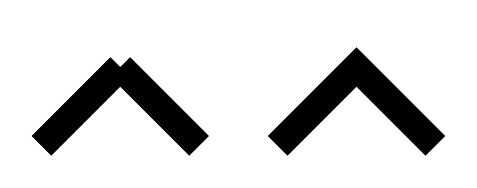
\begin{tikzpicture}[line width=10pt]
  \draw (0,0) --(1,1)  (1,1) --(2,0);
  \draw (3,0) -- (4,1) -- (5,0);
  \useasboundingbox (0,1.5); % make bounding box higher
\end{tikzpicture}
\end{codeexample}

\end{pathoperation}


\subsubsection{Horizontal and Vertical Lines}

Sometimes you want to connect two points via straight lines that are
only horizontal and vertical. For this, you can use two path
construction operations.

{\catcode`\|=12
\begin{pathoperation}[noindex]{-|}{\meta{coordinate}}
  \index{--1@\protect\texttt{-\protect\pgfmanualbar} path operation}%
  \index{Path operations!--1@\protect\texttt{-\protect\pgfmanualbar}}%
  \pgfmanualpdflabel[\catcode`\|=12 ]{-|}{}%
  This operation means ``first horizontal, then vertical.''

  \begin{codeexample}[]
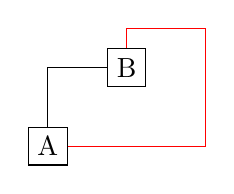
\begin{tikzpicture}
  \draw (0,0) node(a) [draw] {A}  (1,1) node(b) [draw] {B};
  \draw (a.north) |- (b.west);
  \draw[color=red] (a.east) -| (2,1.5) -| (b.north);
\end{tikzpicture}
\end{codeexample}
\end{pathoperation}
\begin{pathoperation}[noindex]{|-}{\meta{coordinate}}
  \index{--2@\protect\texttt{\protect\pgfmanualbar-} path operation}%
  \index{Path operations!--2@\protect\texttt{\protect\pgfmanualbar-}}%
  \pgfmanualpdflabel[\catcode`\|=12 ]{|-}{}%
  This operations means  ``first vertical, then horizontal.''
\end{pathoperation}
}


\subsection{The Curve-To Operation}

The curve-to operation allows you to extend a path using a B�zier
curve.

\begin{pathoperation}{..}{\declare{|controls|}\meta{c}\opt{|and|\meta{d}}\declare{|..|\meta{y}}}
  This operation extends the current path from the current
  point, let us call it $x$, via a curve to a the current point~$y$.
  The curve is a cubic B�zier curve. For such a curve,
  apart from $y$, you also specify two control points $c$ and $d$. The
  idea is that the curve starts at $x$, ``heading'' in the direction
  of~$c$. Mathematically spoken, the tangent of the curve at $x$ goes
  through $c$. Similarly, the curve ends at $y$, ``coming from'' the
  other control point,~$d$. The larger the distance between $x$ and~$c$
  and between $d$ and~$y$, the larger the curve will be.

  If the ``|and|\meta{d}'' part is not given, $d$ is assumed to be
  equal to $c$.

\begin{codeexample}[]
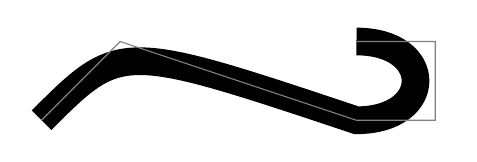
\begin{tikzpicture}
  \draw[line width=10pt] (0,0) .. controls (1,1) .. (4,0)
                               .. controls (5,0) and (5,1) .. (4,1);
  \draw[color=gray] (0,0) -- (1,1) -- (4,0) -- (5,0) -- (5,1) -- (4,1);
\end{tikzpicture}
\end{codeexample}

  As with the line-to operation, it makes a difference whether two curves
  are joined because they resulted from consecutive curve-to or line-to
  operations, or whether they just happen to have the same ending:

\begin{codeexample}[]
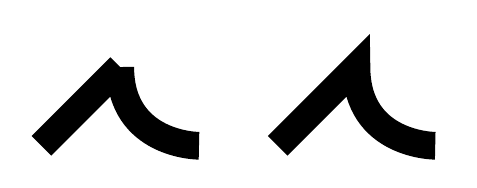
\begin{tikzpicture}[line width=10pt]
  \draw (0,0) -- (1,1) (1,1) .. controls (1,0) and (2,0) .. (2,0);
  \draw (3,0) -- (4,1) .. controls (4,0) and (5,0) .. (5,0);
  \useasboundingbox (0,1.5); % make bounding box higher
\end{tikzpicture}
\end{codeexample}
\end{pathoperation}


\subsection{The Cycle Operation}

\begin{pathoperation}{--cycle}{}
  This operation adds a straight line from the current
  point to the last point specified by a move-to operation. Note that
  this need not be the beginning of the path. Furthermore, a smooth join
  is created between the first segment created after the last move-to
  operation and the straight line appended by the cycle operation.

  Consider the following example. In the left example, two triangles are
  created using three straight lines, but they are not joined at the
  ends. In the second example cycle operations are used.

\begin{codeexample}[]

\begin{tikzpicture}[line width=10pt]
  \draw (0,0) -- (1,1) -- (1,0) -- (0,0) (2,0) -- (3,1) -- (3,0) -- (2,0);
  \draw (5,0) -- (6,1) -- (6,0) -- cycle (7,0) -- (8,1) -- (8,0) -- cycle;
  \useasboundingbox (0,1.5); % make bounding box higher
\end{tikzpicture}
\end{codeexample}
\end{pathoperation}



\subsection{The Rectangle Operation}

A rectangle can obviously be created using four straight lines and a
cycle operation. However, since rectangles are needed so often, a
special syntax is available for them.

\begin{pathoperation}{rectangle}{\meta{corner}}
  When this operation is used, one corner will be the current point,
  another corner is given by \meta{corner}, which becomes the new
  current point.

\begin{codeexample}[]
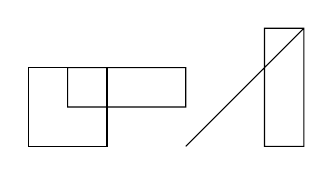
\begin{tikzpicture}
  \draw (0,0) rectangle (1,1);
  \draw (.5,1) rectangle (2,0.5) (3,0) rectangle (3.5,1.5) -- (2,0);
\end{tikzpicture}
\end{codeexample}
\end{pathoperation}


\subsection{Rounding Corners}

All of the path construction operations mentioned up to now are
influenced by the following option:
\begin{key}{/tikz/rounded corners=\meta{inset} (default 4pt)}
  When this option is in force, all corners (places where a line is
  continued either via line-to or a curve-to operation) are replaced by
  little arcs so that the corner becomes smooth.

\begin{codeexample}[]
\tikz \draw [rounded corners] (0,0) -- (1,1)
           -- (2,0) .. controls (3,1) .. (4,0);
\end{codeexample}

  The \meta{inset} describes how big the corner is. Note that the
  \meta{inset} is \emph{not} scaled along if you use a scaling option
  like |scale=2|.

\begin{codeexample}[]
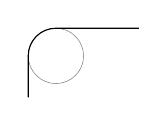
\begin{tikzpicture}
  \draw[color=gray,very thin] (10pt,15pt) circle[radius=10pt];
  \draw[rounded corners=10pt] (0,0) -- (0pt,25pt) -- (40pt,25pt);
\end{tikzpicture}
\end{codeexample}

  You can switch the rounded corners on and off ``in the middle of
  path'' and different corners in the same path can have different
  corner radii:

\begin{codeexample}[]
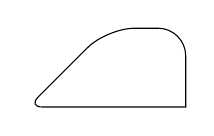
\begin{tikzpicture}
  \draw (0,0) [rounded corners=10pt] -- (1,1) -- (2,1)
                     [sharp corners] -- (2,0)
               [rounded corners=5pt] -- cycle;
\end{tikzpicture}
\end{codeexample}

Here is a rectangle with rounded corners:
\begin{codeexample}[]
\tikz \draw[rounded corners=1ex] (0,0) rectangle (20pt,2ex);
\end{codeexample}

  You should be aware, that there are several pitfalls when using this
  option. First, the rounded corner will only be an arc (part of a
  circle) if the angle is $90^\circ$. In other cases, the rounded
  corner will still be round, but ``not as nice.''

  Second, if there are very short line segments in a path, the
  ``rounding'' may cause inadvertent effects. In such case it may be
  necessary to temporarily switch off the rounding using
  |sharp corners|.
\end{key}

\begin{key}{/tikz/sharp corners}
  This options switches off any rounding on subsequent corners of the
  path.
\end{key}



\subsection{The Circle and Ellipse Operations}

Circles and ellipses are common path elements for which there is a
special path operation.

\begin{pathoperation}{circle}{\opt{|[|\meta{options}|]|}}
  This command adds a circle to the current path where the center of
  the circle is the current point by default, but you can use the |at|
  option to change this. The new current point of the path
  will be (typically just remain) the center of the circle.

  The radius of the circle is specified using the following options:
  \begin{key}{/tikz/x radius=\meta{value}}
    Sets the horizontal radius of the circle (which, when this value
    is different form the vertical radius, is actually an
    ellipse). The \meta{value} may either be a dimension or a
    dimensionless number. In the latter case, the number is
    interpreted in the $xy$-coordinate system (if the $x$-unit is set
    to, say, |2cm|, then |x radius=3| will have the same effect as
    |x radius=6cm|).
  \end{key}
  \begin{key}{/tikz/y radius=\meta{value}}
    Works like the |x radius|.
  \end{key}
  \begin{key}{/tikz/radius=\meta{value}}
    Sets the |x radius| and |y radius| simultaneously.
  \end{key}
  \begin{key}{/tikz/at=\meta{coordinate}}
    If this option is explicitly set inside the \meta{options} (or
    indirectly via the |every circle| style), the \meta{coordinate} is
    used as the center of the circle instead of the current
    point. Setting |at| to some value in an enclosing scope has no
    effect.
  \end{key}
  The \meta{options} may also contain additional options like, say, a
  |rotate| or |scale|, that will only have an effect on the circle.
\begin{codeexample}[]
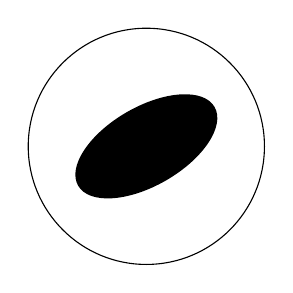
\begin{tikzpicture}
  \draw (1,0) circle [radius=1.5];
  \fill (1,0) circle [x radius=1cm, y radius=5mm, rotate=30];
\end{tikzpicture}
\end{codeexample}

  It is possible to set the |radius| also in some enclosing scope, in
  this case the options can be left out (but see the note below on
  what may follow:
\begin{codeexample}[]
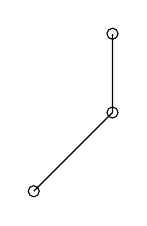
\begin{tikzpicture}[radius=2pt]
  \draw (0,0) circle -- (1,1) circle -- ++(0,1) circle;
\end{tikzpicture}
\end{codeexample}

  The following style is used with every circle:
  \begin{stylekey}{/tikz/every circle}
    You can use this key to setup, say, a default radius for every
    circle. The key will also be used with the |ellipse| operation.
  \end{stylekey}

  In case you feel that the names |radius| and |x radius| are too long
  for your taste, you can easily created shorter aliases:
\begin{codeexample}[code only]
\tikzset{r/.style={radius=#1},rx/.style={x radius=#1},ry/.style={y radius=#1}}
\end{codeexample}
  You can then say |circle [r=1cm]| or |circle [rx=1,ry=1.5]|. The
  reason \tikzname\ uses the longer names by default is that it
  encourages people to write more readable code.

  \emph{Note:} There also exists an older syntax for circles, where
  the radius of the circle is given in parentheses right after the
  |circle| command as in |circle (1pt)|. Although this syntax is a bit
  more succinct, it is harder to understand for readers of the code
  and the use of parentheses for something other than a coordinate is
  ill-chosen.

  \tikzname\ will use the following rule to determine whether the old
  or the normal syntax is used: If |circle| is directly followed by
  something that (expands to) an opening parenthesis, then the old
  syntax is used and inside these following parentheses there must be
  a single number or dimension representing a radius. In all other
  cases the new syntax is used.
\end{pathoperation}

\begin{pathoperation}{ellipse}{|[|\meta{options}|]|}
  This command has exactly the same effect as |circle|. The older
  syntax for this command is |ellipse (|\meta{x radius} |and| \meta{y
    radius}|)|. As for the |circle| command, this syntax is not as
  good as the standard syntax.
\begin{codeexample}[]
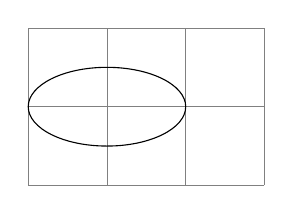
\begin{tikzpicture}
  \draw [help lines] (0,0) grid (3,2);
  \draw (1,1) ellipse [x radius=1cm,y radius=.5cm];
\end{tikzpicture}
\end{codeexample}
\end{pathoperation}



\subsection{The Arc Operation}

The \emph{arc operation} allows you to add an arc to the current
path.
\begin{pathoperation}{arc}{\oarg{options}}
  The |arc| operation adds a part of an ellipse to the current
  path. The radii of the ellipse are given by the values of |x radius|
  and |y radius|, which should be set in the \meta{options}. The arc
  will start at   the current point and will end at the end of the
  arc. The arc  will start and end at angles computed from the three
  keys |start angle|, |end angle|, and |delta angle|. Normally, the
  first two keys specify the start and end angle. However, in case one
  of them is empty, it is computed from the other key plus or minus
  the |delta angle|. In detail, if |end angle| is empty, it is set to
  the start angle plus the delta angle. If the start angle is missing,
  it is set to the end angle minus the delta angle. If all three keys
  are set, the delta angle is ignored.
  \begin{key}{/tikz/start angle=\meta{degrees}}
    Sets the start angle.
  \end{key}
  \begin{key}{/tikz/end angle=\meta{degrees}}
    Sets the end angle.
  \end{key}
  \begin{key}{/tikz/delta angle=\meta{degrees}}
    Sets the delta angle.
  \end{key}

  \begin{codeexample}[]
\begin{tikzpicture}[radius=1cm]
  \draw (0,0)  arc[start angle=180, end angle=90]
     -- (2,.5) arc[start angle=90,  delta angle=-90];
  \draw (4,0) -- +(30:1cm)
              arc [start angle=30,  delta angle=30] -- cycle;
  \draw (8,0) arc [start angle=0,   end angle=270,
                   x radius=1cm, y radius=5mm] -- cycle;
\end{tikzpicture}
\end{codeexample}

\begin{codeexample}[]
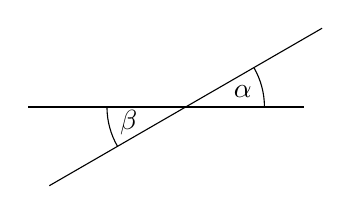
\begin{tikzpicture}[radius=1cm,delta angle=30]
  \draw (-1,0) -- +(3.5,0);
  \draw (1,0) ++(210:2cm) -- +(30:4cm);
  \draw (1,0) +(0:1cm) arc [start angle=0];
  \draw (1,0) +(180:1cm) arc [start angle=180];
  \path (1,0) ++(15:.75cm) node{$\alpha$};
  \path (1,0) ++(15:-.75cm) node{$\beta$};
\end{tikzpicture}
\end{codeexample}

  There also exists a shorter syntax for the arc operation, namely
  |arc| begin directly followed by |(|\meta{start angle}|:|\meta{end
    angle}|:|\meta{radius}). However, this syntax is harder to read,
  so the normal syntax should be preferred in general.
\end{pathoperation}


\subsection{The Grid Operation}

You can add a grid to the current path using the |grid| path
operation.

\begin{pathoperation}{grid}{\opt{\oarg{options}}\meta{corner}}
  This operations adds a grid filling a rectangle whose two corners
  are given by \meta{corner} and by the previous coordinate. Thus, the
  typical way in which a grid is drawn is |\draw (1,1) grid (3,3);|,
  which yields a grid filling the rectangle whose corners are at
  $(1,1)$ and $(3,3)$. All coordinate transformations apply to the
  grid.

\begin{codeexample}[]
\tikz[rotate=30] \draw[step=1mm] (0,0) grid (2,2);
\end{codeexample}

  The \meta{options}, which are local to the |grid| operation, can be
  used to influence the appearance of the grid. The stepping of the
  grid is governed by the following options:

\begin{key}{/tikz/step=\meta{number or dimension or coordinate}
    (initially 1cm)}
  Sets the stepping in both the
  $x$ and $y$-direction. If a dimension is provided, this is used
  directly. If a number is provided, this number is interpreted in the
  $xy$-coordinate system. For example, if you provide the number |2|,
  then the $x$-step is twice the $x$-vector and the $y$-step is twice
  the $y$-vector set by the |x=| and |y=| options. Finally, if you
  provide a coordinate, then the $x$-part of this coordinate will be
  used as the $x$-step and the $y$-part will be used as the
  $y$-coordinate.

\begin{codeexample}[]
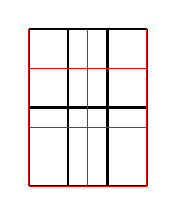
\begin{tikzpicture}[x=.5cm]
  \draw[thick] (0,0) grid [step=1]     (3,2);
  \draw[red]   (0,0) grid [step=.75cm] (3,2);
\end{tikzpicture}
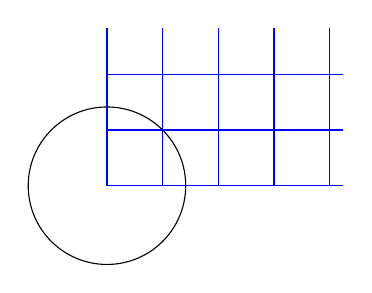
\begin{tikzpicture}
  \draw        (0,0) circle [radius=1];
  \draw[blue]  (0,0) grid [step=(45:1)] (3,2);
\end{tikzpicture}
\end{codeexample}

  A complication arises when the $x$- and/or $y$-vector do not point
  along the axes. Because of this, the actual rule for computing the
  $x$-step and the $y$-step is the following: As the $x$- and
  $y$-steps we use the $x$- and $y$-components or the following two
  vectors: The first vector is either $(\meta{x-grid-step-number},0)$
  or $(\meta{x-grid-step-dimension},0\mathrm{pt})$, the second vector
  is  $(0,\meta{y-grid-step-number})$ or
  $(0\mathrm{pt},\meta{x-grid-step-dimension})$.
\end{key}

\begin{key}{/tikz/xstep=\meta{dimension or number} (initially 1cm)}
  Sets the stepping in the $x$-direction.
\begin{codeexample}[]
\tikz \draw (0,0) grid [xstep=.5,ystep=.75] (3,2);
\end{codeexample}
\end{key}

\begin{key}{/tikz/ystep=\meta{dimension or number} (initially 1cm)}
  Sets the stepping in the $y$-direction.
\end{key}

  It is important to note that the grid is always ``phased'' such that
  it contains the point $(0,0)$ if that point happens to be inside the
  rectangle. Thus, the grid does \emph{not} always have an intersection
  at the corner points; this occurs only if the corner points are
  multiples of the stepping. Note that due to rounding errors, the
  ``last'' lines of a grid may be omitted. In this case, you have to
  add an epsilon to the corner points.

  The following style is useful for drawing grids:
\begin{stylekey}{/tikz/help lines (initially {line width=0.2pt,gray})}
  This style makes lines ``subdued'' by using thin gray lines for
  them. However, this style is not installed automatically and you
  have to say for example:
\begin{codeexample}[]
\tikz \draw[help lines] (0,0) grid (3,3);
\end{codeexample}
\end{stylekey}

\end{pathoperation}



\subsection{The Parabola Operation}

The |parabola| path operation continues the current path with a
parabola. A parabola is a (shifted and scaled) curve defined by the
equation $f(x) = x^2$ and looks like this: \tikz \draw (-1ex,1.5ex)
parabola[parabola height=-1.5ex] +(2ex,0ex);.

\begin{pathoperation}{parabola}{\opt{\oarg{options}|bend|\meta{bend
        coordinate}}\meta{coordinate}}
  This operation adds a parabola through the current point and the
  given \meta{coordinate}. If the |bend| is given, it specifies where
  the bend should go; the \meta{options} can also be used to specify
  where the bend is. By default, the bend is at the old current point.

\begin{codeexample}[]
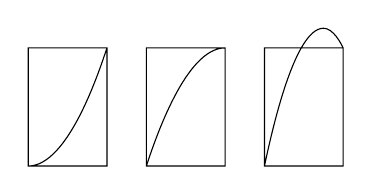
\begin{tikzpicture}
  \draw               (0,0) rectangle                (1,1.5)
                      (0,0) parabola                 (1,1.5);
  \draw[xshift=1.5cm] (0,0) rectangle                (1,1.5)
                      (0,0) parabola[bend at end]    (1,1.5);
  \draw[xshift=3cm]   (0,0) rectangle                (1,1.5)
                      (0,0) parabola bend (.75,1.75) (1,1.5);
\end{tikzpicture}
\end{codeexample}

  The following options influence parabolas:
\begin{key}{/tikz/bend=\meta{coordinate}}
  Has the same effect as saying |bend|\meta{coordinate} outside the
  \meta{options}. The option specifies that the bend of the parabola
  should be at the given \meta{coordinate}. You have to take care
  yourself that the bend position is a ``valid'' position; which means
  that if there is no parabola of the form $f(x) = a x^2 + b x + c$
  that goes through the old current point, the given bend, and the new
  current point, the result will not be a parabola.

  There is one special property of the \meta{coordinate}: When a
  relative coordinate is given like |+(0,0)|, the position relative
  to which this coordinate is ``flexible.'' More precisely, this
  position lies somewhere on a line from the old current point to the
  new current point. The exact position depends on the next
  option.
\end{key}

\begin{key}{/tikz/bend pos=\meta{fraction}}
  Specifies where the ``previous'' point is relative to which the bend
  is calculated. The previous point will be at the \meta{fraction}th
  part of the line from the old current point to the new current
  point.

  The idea is the following: If you say |bend pos=0| and
  |bend +(0,0)|, the bend will be at the old current point. If you say
  |bend pos=1| and |bend +(0,0)|, the bend will be at the new current
  point. If you say |bend pos=0.5| and |bend +(0,2cm)| the bend will
  be 2cm above the middle of the line between the start and end
  point. This is most useful in situations such as the following:
\begin{codeexample}[]
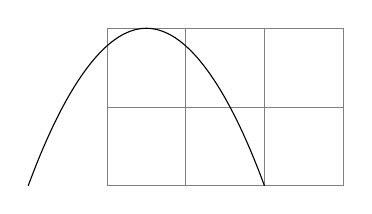
\begin{tikzpicture}
  \draw[help lines] (0,0) grid (3,2);
  \draw (-1,0) parabola[bend pos=0.5] bend +(0,2) +(3,0);
\end{tikzpicture}
\end{codeexample}

  In the above example, the |bend +(0,2)| essentially means ``a
  parabola that is 2cm high'' and |+(3,0)| means ``and 3cm wide.''
  Since this situation arises often, there is a special shortcut
  option:
  \begin{key}{/tikz/parabola height=\meta{dimension}}
    This option has the same effect as
    |[bend pos=0.5,bend={+(0pt,|\meta{dimension}|)}]|.
\begin{codeexample}[]
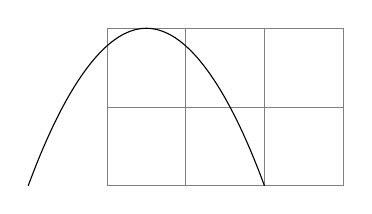
\begin{tikzpicture}
  \draw[help lines] (0,0) grid (3,2);
  \draw (-1,0) parabola[parabola height=2cm] +(3,0);
\end{tikzpicture}
\end{codeexample}
  \end{key}
\end{key}

The following styles are useful shortcuts:
\begin{stylekey}{/tikz/bend at start}
  This places the bend at the start of a
  parabola. It is a shortcut for the following options:
  |bend pos=0,bend={+(0,0)}|.
\end{stylekey}

\begin{stylekey}{/tikz/bend at end}
  This places the bend at the end of a parabola.
\end{stylekey}

\end{pathoperation}


\subsection{The Sine and Cosine Operation}

The |sin| and |cos| operations are similar to the |parabola|
operation. They, too, can be used to draw (parts of) a sine or cosine
curve.

\begin{pathoperation}{sin}{\meta{coordinate}}
  The effect of |sin| is to draw a scaled and shifted version of a sine
  curve in the interval $[0,\pi/2]$. The scaling and shifting is done in
  such a way that the start of the sine curve in the interval is at the
  old current point and that the end of the curve in the interval is at
  \meta{coordinate}. Here is an example that should clarify this:

\begin{codeexample}[]
\tikz \draw (0,0) rectangle (1,1)     (0,0) sin (1,1)
            (2,0) rectangle +(1.57,1) (2,0) sin +(1.57,1);
\end{codeexample}
\end{pathoperation}

\begin{pathoperation}{cos}{\meta{coordinate}}
  This operation works similarly, only a cosine in the interval
  $[0,\pi/2]$ is drawn. By correctly alternating |sin| and |cos|
  operations, you can create a complete sine or cosine curve:

\begin{codeexample}[]
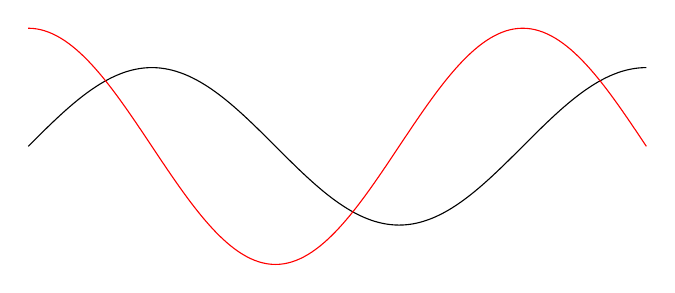
\begin{tikzpicture}[xscale=1.57]
  \draw (0,0) sin (1,1) cos (2,0) sin (3,-1) cos (4,0) sin (5,1);
  \draw[color=red] (0,1.5) cos (1,0) sin (2,-1.5) cos (3,0) sin (4,1.5) cos (5,0);
\end{tikzpicture}
\end{codeexample}
\end{pathoperation}

Note that there is no way to (conveniently) draw an interval on a sine
or cosine curve whose end points are not multiples of $\pi/2$.


\subsection{The SVG Operation}

The |svg| operation can be used to extend the current path by a path
given in the \textsc{svg} path data syntax. This syntax is described
in detail in Section 8.3 of the \textsc{svg 1.1} specification, please
consult this specification for details.

\begin{pathoperation}{svg}{\opt{\oarg{options}}|"|\meta{path data}|"|}
  This operation adds the path specified in the \meta{path data} in
  \textsc{svg 1.1 path data} syntax to the current path. Unlike the
  \textsc{svg}-specification, it \emph{is} permissible that the path
  data does not start with a moveto command (|m| or |M|), in which
  case the last point of the current path is used as start point.
  The optional \meta{options} apply locally to this path operation,
  typically you will use them to setup, say, some transformations.

\begin{codeexample}[]
\begin{tikzpicture}
  \filldraw [fill=red!20] (0,1) svg[scale=2] "h 10 v 10 h -10"
    node [above left] {upper left} -- cycle;

  \draw svg "M 0 0 L 20 20 h 10 a 10 10 0 0 0 -20 0";
\end{tikzpicture}
\end{codeexample}

  An \textsc{svg} coordinate like |10 20| is always interpreted as
  |(10pt,20pt)|, so the basic unit is always points (|pt|). The
  $xy$-coordinate system is not used. However, you can use scaling to
  (locally) change the basic unit. For instance, |svg[scale=1cm]|
  (yes, this works, although some rather evil magic is involved) will
  cause 1cm to be the basic unit.

  \emph{Warning:} The arc operations (|a| and |A|) are not numerically
  stable. This means that they will be quite imprecise, except when
  the angle is a multiple of $90^\circ$ (as is, fortunately, most
  often the case).
\end{pathoperation}

\subsection{The Plot Operation}

The |plot| operation can be used to append a line or curve to the path
that goes through a large number of coordinates. These coordinates are
either given in a simple list of coordinates, read from some file, or
they are computed on the fly.

Since the syntax and the behaviour of this command are a bit complex,
they are described in the separated Section~\ref{section-tikz-plots}.

\subsection{The To Path Operation}

The |to| operation is used to add a user-defined path
from the previous coordinate to the following coordinate. When you
write |(a) to (b)|, a straight line is added from |a|
to |b|, exactly as if you had written |(a) -- (b)|. However, if you
write |(a) to [out=135,in=45] (b)| a curve is added to the path,
which leaves at an angle of 135$^\circ$ at |a| and arrives at an angle
of 45$^\circ$ at |b|. This is because the options |in| and |out|
trigger a special path to be used instead of the straight line.

\begin{pathoperation}{to}{\opt{|[|\meta{options}|]|}
    \opt{\meta{nodes}} |(|\meta{coordinate}|)|}

  This path operation inserts the path current set via the |to path|
  option at the current position. The \meta{options} can be used to
  modify (perhaps implicitly) the |to path| and to setup how the path
  will be rendered.

  Before the |to path| is inserted, a number of macros are setup that
  can ``help'' the |to path|. These are |\tikztostart|,
  |\tikztotarget|, and |\tikztonodes|; they are explained in the
  following.

  \medskip
  \textbf{Start and Target Coordinates.}\ \
  The |to| operation is always followed by a \meta{coordinate}, called
  the target coordinate. The macro |\tikztotarget| is set to this
  coordinate (without the parentheses). There is also a \emph{start
    coordinate}, which is the coordinate preceding the |to|
  operation. This coordinate can be accessed via the macro
  |\tikztostart|. In the following example, for the first |to|, the
  macro |\tikztostart| is |0pt,0pt| and the |\tikztotarget| is
  |0,2|. For the second |to|, the macro |\tikztostart| is |10pt,10pt|
  and |\tikztotarget| is |a|.

\begin{codeexample}[]
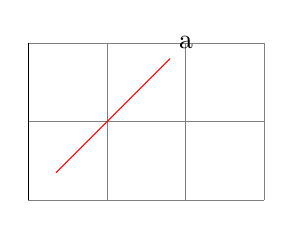
\begin{tikzpicture}
  \draw[help lines] (0,0) grid (3,2);

  \draw      (0,0)       to (0,2);
  \node      (a)         at (2,2) {a};
  \draw[red] (10pt,10pt) to (a);
\end{tikzpicture}
\end{codeexample}


  \medskip
  \textbf{Nodes on tos.}\ \
  It is possible to add nodes to the paths constructed by a |to|
  operation. To do so, you specify the nodes between the |to|
  keyword and the coordinate (if there are options to the |to|
  operation, these come first). The effect of |(a) to node {x} (b)|
  (typically) is the same as if you had written
  |(a) -- node {x} (b)|, namely that the node is placed on the
  to. This can be used to add labels to tos:

\begin{codeexample}[]
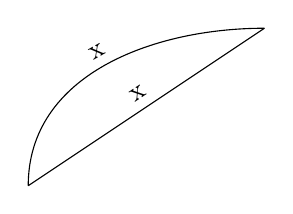
\begin{tikzpicture}
  \draw (0,0) to node [sloped,above] {x} (3,2);

  \draw (0,0) to[out=90,in=180] node [sloped,above] {x} (3,2);
\end{tikzpicture}
\end{codeexample}

  \medskip
  \textbf{Styles for to-paths.}\ \
  In addition to the \meta{options} given after the |to| operation,
  the following style is also set at the beginning of the to path:
  \begin{stylekey}{/tikz/every to (initially \normalfont empty)}
    This style is installed at the beginning of every to.
\begin{codeexample}[]
\tikz[every to/.style={bend left}]
  \draw (0,0) to (3,2);
\end{codeexample}
  \end{stylekey}

  \medskip
  \textbf{Options.}\ \
  The \meta{options} given with the |to| allow you to influence the
  appearance of the |to path|. Mostly, these options are used to
  change the |to path|. This can be used to change the path from a
  straight line to, say, a curve.

  The path used is set using the following option:
  \begin{key}{/tikz/to path=\meta{path}}
    Whenever an |to| operation is used, the \meta{path} is
    inserted. More precisely, the following path is added:

    \begin{quote}
      |{[every to,|\meta{options}|] |\meta{path} |}|
    \end{quote}

    The \meta{options} are the options given to the |to| operation,
    the \meta{path} is the path set by this option |to path|.

    Inside the \meta{path}, different macros are used to reference the
    from- and to-coordinates. In detail, these are:
    \begin{itemize}
    \item \declare{|\tikztostart|} will expand to the from-coordinate
      (without the parentheses).
    \item \declare{|\tikztotarget|} will expand to the to-coordinate.
    \item \declare{|\tikztonodes|} will expand to the nodes between
      the |to| operation and the coordinate. Furthermore, these
      nodes will have the |pos| option set implicitly.
    \end{itemize}

    Let us have a look at a simple example. The standard straight line
    for an to is achieved by the following \meta{path}:
    \begin{quote}
      |-- (\tikztotarget) \tikztonodes|
    \end{quote}

    Indeed, this is the default setting for the path. When we write
    |(a) to (b)|, the \meta{path} will expand to |(a) -- (b)|, when
    we write
    \begin{quote}
      |(a) to[red] node {x} (b)|
    \end{quote}
    the \meta{path} will expand to
    \begin{quote}
      |(a) -- (b) node[pos] {x}|
    \end{quote}

    It is not possible to specify the path
    \begin{quote}
      |-- \tikztonodes (\tikztotarget)|
    \end{quote}
    since \tikzname\ does not allow one to have a macro after |--|
    that expands to a node.

    Now let us have a look at how we can modify the \meta{path}
    sensibly. The simplest way is to use a curve.

\begin{codeexample}[]
\begin{tikzpicture}[to path={
    .. controls +(1,0) and +(1,0) .. (\tikztotarget) \tikztonodes}]

  \node (a) at (0,0) {a};
  \node (b) at (2,1) {b};
  \node (c) at (1,2) {c};

  \draw (a) to node {x} (b)
        (a) to          (c);
\end{tikzpicture}
\end{codeexample}

    Here is another example:

\begin{codeexample}[]
\tikzset{
  my loop/.style={to path={
    .. controls +(80:1) and +(100:1) .. (\tikztotarget) \tikztonodes}},
  my state/.style={circle,draw}}

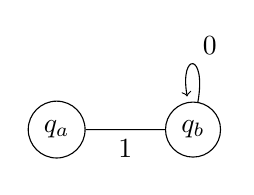
\begin{tikzpicture}[shorten >=2pt]
  \node [my state] (a) at (210:1) {$q_a$};
  \node [my state] (b) at (330:1) {$q_b$};

  \draw[->] (a) to           node[below]       {1} (b)
                to [my loop] node[above right] {0} (b);
\end{tikzpicture}
\end{codeexample}

    \begin{key}{/tikz/execute at begin to=\meta{code}}
      The \meta{code} is executed prior to the to. This can be used to
      draw one or more additional paths or to do additional
      computations.
    \end{key}

    \begin{key}{/tikz/execute at end to=\meta{code}}
      Works like the previous option, only this code is executed after
      the to path has been added.
	  % FIXME : provide examples...
    \end{key}


    \begin{stylekey}{/tikz/every to (initially \normalfont empty)}
      This style is installed at the beginning of every to.
    \end{stylekey}
  \end{key}
\end{pathoperation}

There are a number of predefined |to path|s, see
Section~\ref{library-to-paths} for a reference.


\subsection{The Let Operation}

The \emph{let operation} is the first of a number of path operations
that do not actually extend that path, but have different, mostly
local, effects.

\begin{pathoperation}{let}{\meta{assignment}
    \opt{|,|\meta{assignment}}%
    \opt{|,|\meta{assignment}\dots}\declare{| in |}}
  When this path operation is encountered, the \meta{assignment}s are
  evaluated, one by one. This will store coordinate and number in
  special \emph{registers} (which are local to \tikzname, they have
  nothing to do with \TeX\ registers). Subsequently, one can access the
  contents of these registers using the macros |\p|, |\x|, |\y|, and
  |\n|.

  The first kind of permissible \meta{assignment}s have the following
  form:
  \begin{quote}
    |\n|\meta{number register}|={|\meta{formula}|}|
  \end{quote}
  When an assignment has this form, the \meta{formula} is evaluated
  using the |\pgfmathparse| operation. The result stored in the
  \meta{number register}. If the \meta{formula} involves a dimension
  anywhere (as in |2*3cm/2|), then the \meta{number register} stores
  the resulting dimension with a trailing |pt|.  A \meta{number register} can
  be named arbitrarily and is a normal \TeX\  parameter to the |\n|
  macro. Possible names are |{left corner}|, but also just a single
  digit like~|5|.

  Let us call the path that follows a let operation its
  \emph{body}. Inside the body, the |\n| macro can be used to access
  the register.
  \begin{command}{\n\marg{number register}}
    When this macro is used on the left-hand side of an |=|-sign in a
    let operation, it has no effect and is just there for
    readability. When the macro is used on the right-hand side of an
    |=|-sign or in the body of the let operation, then it expands to
    the value stored in the \meta{number register}. This will either
    be a dimensionless number like |2.0| or a dimension like |5.6pt|.

    For instance, if we say |let \n1={1pt+2pt}, \n2={1+2} in ...|, then
    inside the |...| part the macro |\n1| will expand to |3pt| and
    |\n2| expands to |3|.
  \end{command}

  The second kind of \meta{assignments} have the following form:
  \begin{quote}
    |\p|\meta{point register}|={|\meta{formula}|}|
  \end{quote}
  Point position registers store a single point, consisting
  of an $x$-part and a $y$-part measured in \TeX\ points (|pt|). In
  particular, point registers do not stored nodes or node names.
  Here is an example:
\begin{codeexample}[]
\begin{tikzpicture}
  \draw [help lines] (0,0) grid (3,2);

  \draw let \p{foo} = (1,1), \p2 = (2,0) in
          (0,0) -- (\p2) -- (\p{foo});
\end{tikzpicture}
\end{codeexample}

  \begin{command}{\p\marg{point register}}
    When this macro is used on the left-hand side of an |=|-sign in a
    let operation, it has no effect and is just there for
    readability. When the macro is used on the right-hand side of an
    |=|-sign or in the body of the let operation, then it expands to
    the $x$-part (measured in \TeX\ points) of the coordinate stored
    in the \meta{register}, followed, by a comma, followed by the
    $y$-part.

    For instance, if we say |let \p1=(1pt,1pt+2pt) in ...|, then
    inside the |...| part the macro |\p1| will expand to exactly the
    seven characters ``1pt,3pt''. This means that you when you write
    |(\p1)|, this expands to |(1pt,3pt)|, which is presumably exactly
    what you intended.
  \end{command}
  \begin{command}{\x\marg{point register}}
    This macro expand just to the $x$-part of the point
    register. If we say as above, as we did above,
    |let \p1=(1pt,1pt+2pt) in ...|, then
    inside the |...| part the macro |\x1| expands to |1pt|.
  \end{command}
  \begin{command}{\y\marg{point register}}
    Works like |\x|, only for the $y$-part.
  \end{command}
  Note that the above macros are available only inside a let
  operation.

  Here is an example where let clauses are used to assemble a coordinate
  from the $x$-coordinate of a first point and the $y$-coordinate of a
  second point. Naturally, using the \verb!|-! notation, this could be
  written much more compactly.
\begin{codeexample}[]
\begin{tikzpicture}
  \draw [help lines] (0,0) grid (3,2);

  \draw    (1,0) coordinate (first point)
        -- (3,2) coordinate (second point);

  \fill[red] let \p1 = (first point),
                 \p2 = (second point) in
               (\x1,\y2) circle [radius=2pt];
\end{tikzpicture}
\end{codeexample}

  Note that the effect of a let operation is local to the body of the
  let operation. If you wish to access a computed coordinate outside
  the body, you must use a |coordinate| path operation:
\begin{codeexample}[]
\begin{tikzpicture}
  \draw [help lines] (0,0) grid (3,2);

  \path % let's define some points:
    let
      \p1        = (1,0),
      \p2        = (3,2),
      \p{center} = ($ (\p1) !.5! (\p2) $) % center
    in
      coordinate (p1) at (\p1)
      coordinate (p2) at (\p2)
      coordinate (center) at (\p{center});

  \draw (p1) -- (p2);
  \fill[red] (center) circle [radius=2pt];
\end{tikzpicture}
\end{codeexample}

  For a more useful application of the let operation, let use draw a
  circle that touches a given line:
\begin{codeexample}[]
\begin{tikzpicture}
  \draw [help lines] (0,0) grid (3,3);

  \coordinate (a) at (rnd,rnd);
  \coordinate (b) at (3-rnd,3-rnd);
  \draw (a) -- (b);

  \node (c) at (1,2) {x};

  \draw let \p1 = ($ (a)!(c)!(b) - (c) $),
            \n1 = {veclen(\x1,\y1)}
        in circle [at=(c), radius=\n1];
\end{tikzpicture}
\end{codeexample}
\end{pathoperation}


\subsection{The Scoping Operation}

When \tikzname\ encounters and opening or a closing brace (|{| or~|}|) at
some point where a path operation should come, it will open or close a
scope. All options that can be applied ``locally'' will be scoped
inside the scope. For example, if you apply a transformation like
|[xshift=1cm]| inside the scoped area, the shifting only applies to
the scope. On the other hand, an option like |color=red| does not have
any effect inside a scope since it can only be applied to the path as
a whole.

Concerning the effect of scopes on relative coordinates,
please see Section~\ref{section-scopes-relative}.


\subsection{The Node and Edge Operations}

There are two more operations that can be found in paths:
|node| and |edge|. The first is used to add a so-called node to a
path. This operation is special in the following sense: It does not
change the current path in any way. In other words, this operation
is not really a path operation, but has an effect that is
``external''  to the path. The |edge| operation has similar effect in
that it adds something \emph{after} the main path has been
drawn. However, it works like the |to| operation, that is, it adds a
|to| path to the picture after the main path has been drawn.

Since these operations are quite complex, they are described in the
separate Section~\ref{section-nodes}.



\subsection{The PGF-Extra Operation}

In some cases you may need to ``do some calculations or some other
stuff'' while a path is constructed. For this, you would like to
suspend the construction of the path and suspend \tikzname's parsing
of the path, you would then like to have some \TeX\ code executed, and
would then like to resume the parsing of the path. This effect can be
achieved using the following path operation |\pgfextra|. Note that
this operation should only be used by real experts and should only be
used deep inside clever macros, not on normal paths.

\begin{command}{\pgfextra\marg{code}}
  This command may only be used inside a \tikzname\ path. There it is
  used like a normal path operation. The construction of the path is
  temporarily suspended and the \meta{code} is executed. Then, the
  path construction is resumed.

\begin{codeexample}[]
\newdimen\mydim
\begin{tikzpicture}
  \mydim=1cm
  \draw (0pt,\mydim) \pgfextra{\mydim=2cm} -- (0pt,\mydim);
\end{tikzpicture}
\end{codeexample}
\end{command}

\begin{command}{\pgfextra \meta{code} \texttt{\char`\\endpgfextra}}
  This is an alternative syntax for the |\pgfextra| command. If the
  code following |\pgfextra| does not start with a brace, the
  \meta{code} is executed until |\endpgfextra| is encountered. What
  actually happens is that |\pgfextra| that is not followed by a brace
  completely shuts down the \tikzname\ parse and |\endpgfextra| is a
  normal macro that restarts the parser.

\begin{codeexample}[]
\newdimen\mydim
\begin{tikzpicture}
  \mydim=1cm
  \draw (0pt,\mydim)
    \pgfextra \mydim=2cm \endpgfextra -- (0pt,\mydim);
\end{tikzpicture}
\end{codeexample}
\end{command}
